\chapter{Задание}

\section{Условие}
Запрограммировать демона и проанализировать информацию об этом процессе.

\section{Реализация}

\begin{lstlisting}
#include <sys/resource.h>
#include <sys/types.h>
#include <sys/file.h>
#include <sys/stat.h>

#include <unistd.h>
#include <signal.h>
#include <syslog.h>
#include <fcntl.h>

#include <stdlib.h>
#include <string.h>
#include <stdio.h>
#include <errno.h>
#include <time.h>

#define LOCK_FILE "/var/run/daemon.pid"
#define LOCK_MODE (S_IRUSR | S_IWUSR | S_IRGRP | S_IROTH)

int already_running(void);
void daemonize(const char *cmd);

int main(int argc, const char **argv)
{
    daemonize(argv[0]);

    if (already_running())
    {
        syslog(LOG_ERR, "Daemon is already running");
        exit(1);
    }

    time_t time_var;

    for (;;)
    {
        time_var = time(NULL);
        syslog(LOG_INFO, "Time: %s\n", ctime(&time_var));

        sleep(5);
    }
}

void daemonize(const char *cmd)
{
    // 1 правило:
    // для возможности создания файлов с любыми правами доступа
    // сброс маски режима создания файла
    umask(0);

    pid_t pid;
    struct rlimit rl;
    struct sigaction sa;

    // Получить максимально возможный номер дескриптора файла
    if (getrlimit(RLIMIT_NOFILE, &rl) < 0)
    {
        fprintf(stderr, "%s: getrlimit, %s\n", cmd, strerror(errno));
        exit(1);
    }

    // 2 правило:
    // создание дочернего процесса и завершение процесса-предка
    if ((pid = fork()) < 0)
    {
        fprintf(stderr, "%s: fork, %s\n", cmd, strerror(errno));
        exit(1);
    }
    else if (pid != 0)
    {
        exit(0);
    }

    // 3 правило:
    // обеспечение невозможности обретения
    // управляющего терминала в будущем
    setsid();

    sa.sa_handler = SIG_IGN;
    sigemptyset(&sa.sa_mask);
    sa.sa_flags = 0;

    if (sigaction(SIGHUP, &sa, NULL) < 0)
    {
        fprintf(stderr, "%s: can not ignore SIGHUP, %s\n",
                cmd, strerror(errno));
        exit(1);
    }

    // 4 правило:
    // Назначение корневого каталога текущим рабочим каталогом
    // (на случай, если демон был запущен с  подмонтированной ФС)
    if (chdir("/") < 0)
    {
        fprintf(stderr, "%s: can not cd to \"/\", %s\n",
                cmd, strerror(errno));
        exit(1);
    }

    // 5 правило:
    // Закрытие всех открытх файловых дескрипторов
    if (rl.rlim_max == RLIM_INFINITY)
    {
        rl.rlim_max = 1024;
    }

    for (int i = 0; i < rl.rlim_max; ++i)
    {
        close(i);
    }

    // 6 правило:
    // Присоединение файловых дескрипторов 1, 2, 3 к /deb/null
    int fd0 = open("/dev/null", O_RDWR);
    int fd1 = dup(0);
    int fd2 = dup(0);

    // Инициализация файла журнала
    openlog(cmd, LOG_CONS, LOG_DAEMON);

    if (fd0 != 0 || fd1 != 1 || fd2 != 2)
    {
        syslog(LOG_ERR, "Wrong file descriptors %d %d %d", fd0, fd1, fd2);
        exit(1);
    }
}

int already_running(void)
{
    int fd;
    char buf[256];

    fd = open(LOCK_FILE, O_RDWR | O_CREAT, LOCK_MODE);

    if (fd < 0)
    {
        syslog(LOG_ERR, "Can not be open %s: %s",
               LOCK_FILE, strerror(errno));
        exit(1);
    }

    // Если файл уже заблокирован
    if (flock(fd, LOCK_EX | LOCK_NB) < 0)
    {
        if (errno == EWOULDBLOCK)
        {
            close(fd);
            return 1;
        }

        syslog(LOG_ERR, "Can not block %s: %s",
               LOCK_FILE, strerror(errno));
        exit(1);
    }

    ftruncate(fd, 0);
    sprintf(buf, "%d", getpid());
    write(fd, buf, strlen(buf) + 1);

    return 0;
}
\end{lstlisting}

\section{Анализ информации о процессе-демоне}
Запустим программу с правами супер-пользователя и выведем информацию о процессах в системе, используя команду ps с ключами ---a (вывод процессов, которыми владеют другие пользователи), ---j (вывод идентификаторов сессии, группы процессов, управляющего терминала и группы процессов терминала) и ---x (вывод процессов, не имеющих управляющего терминала).
\begin{figure}[H]
    \centering
    \caption{}
    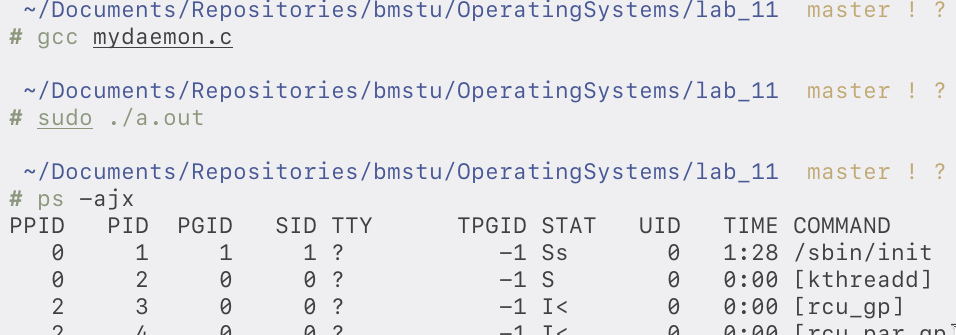
\includegraphics[scale=.4]{images/scr_01.png}
\end{figure}

Колонки, слева направо: идентификатор родительского процесса, идентификатор процесса, идентификатор группы процессов, идентификатор сессии, имя терминала, идентификатор группы процессов терминала, состояние процесса, идентификатор пользователя, совокупное время использования процессора для конкретного процесса и строка команды.

\begin{figure}[H]
    \centering
    \caption{}
    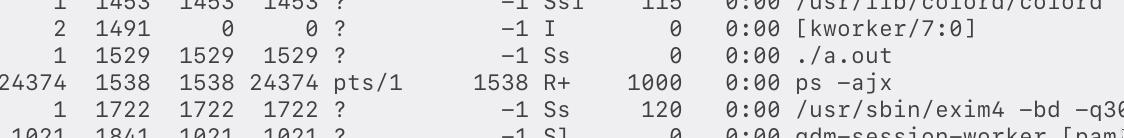
\includegraphics[scale=.4]{images/scr_02.png}
\end{figure}

Процесс демон имеет идентификатор 1529. Кроме того, у него совпадают идентификаторы процесса, лидера сессии, лидера группы, потому что процесс-демон является лидером группы и лидером сессии, единственным в своей группе и сессии. В колонке имени терминала стоит знак вопроса, что означает, у процесса-демона нет управляющего терминала. Состояние процесса~--- Ss. S означает прерываемый сон, а s~--- процесс является лидером сессии.

Процесс-демон не может выводить сообщения на стандартное устройство вывода сообщений об ошибках, так как он не имеет управляющего терминала. Поэтому для вывода сообщений используется механизм syslog. Эта функция отправляет сообщения через сокет домена UNIX~--- /dev/log.

Используя команду sudo tail -f /var/log/syslog, получим последнее содержимое syslog. Затем попробуем запустить демона еще раз~--- в syslog выведется предупреждение, что этот демон уже запущен (так как он должен быть единственным в своей группе и сессии).

\begin{figure}[H]
    \centering
    \caption{}
    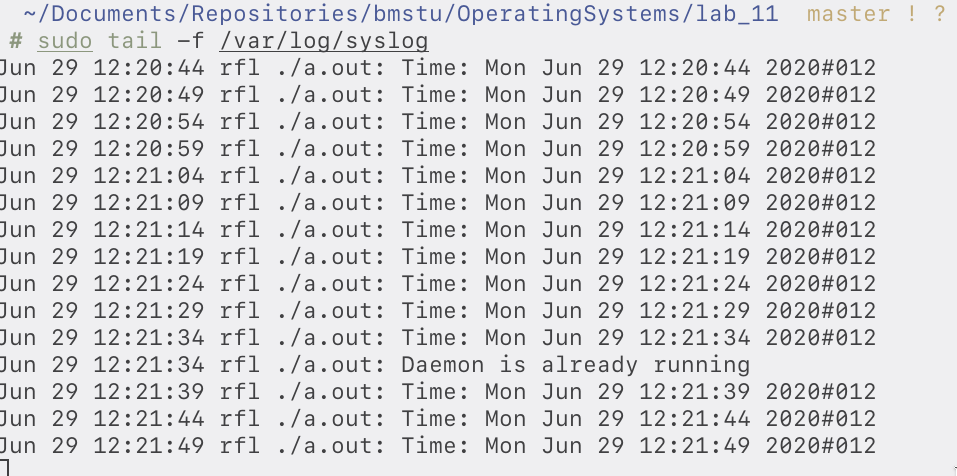
\includegraphics[scale=.4]{images/scr_03.png}
\end{figure}

Убьем демона при помощи команды sudo kill и увидим, что он пропал из списка процессов:

\begin{figure}[H]
    \centering
    \caption{}
    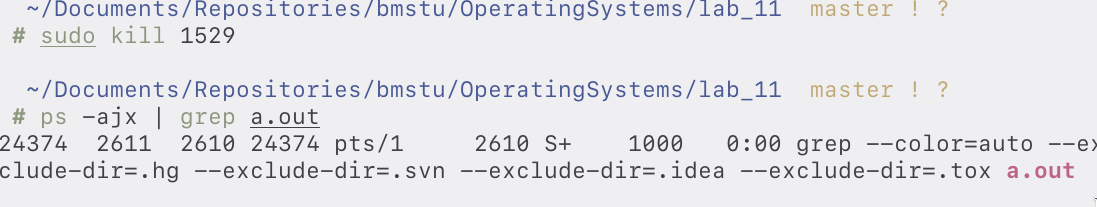
\includegraphics[scale=.4]{images/scr_04.png}
\end{figure}
